\documentclass[../Paper.tex]{subfiles}

\begin{document}

\section{List of Symbols}

\renewcommand\arraystretch{1.5} % <-- 设置表格行高
\begin{table}[H]
\centering
\scriptsize %此处写字体大小控制命令
\begin{tabular}{p{2cm}<{\centering} p{6.5cm}<{\centering} p{3cm}<{\centering} %p{1cm}<{\centering} p{1cm}<{\centering} 
				p{1cm}<{\centering} p{1cm}<{\centering} }
		\hline
Symbol & Description & Value \\
	    \hline
	    \hline
$S.$ & Solar constant/W$\cdot s^{-2}$ & 1367 \\

$G$ & Universal gravitational constant/$m^3kg^{-1}s^{-2}$ & $6.67259\times10^{-11}$ \\

$R_E$ & The distance from the sun to the earth/m & $1.496\times10^{11}$ \\
		
$R_M$ & The distance from the sun to the Mars/m & $2.2794\times10^{11}$ \\

$M_S$ & The masse of the sun/kg & $1.9891\times10^{30}$  \\

$M_E$ & The masse of the earth/kg & $5.965\times10^{24}$  \\

$M_M$ & The masse of the Mars/kg & $6.4219\times10^{23}$  \\

$m$ & Total mass (sail plus payload)/kg & 2000~ \\

$T_E$ & The period of revolution of earth/s & $3.1536\times10^{7}$~(365days) \\

$T_M$ & The period of revolution of Mars/s & $5.93568\times10^{7}$~(687days)\\

$\omega_E$ & The angular velocity of revolution of earth/rad$\cdot s^{-1}$ & $1.9924\times10^{-7}$ \\

$\omega_M$ & The angular velocity of revolution of Mars/rad$\cdot s^{-1}$ & $1.0585\times10^{-7}$ \\

$\alpha$ & The attitude angle of solar sail & $-\dfrac{\pi}{2}\leq\alpha\leq\dfrac{\pi}{2}$ \\

$A$ & The area of solar sail &  \\
	    \hline
\end{tabular}

\caption{List of symbols}
\label{Table1}
\end{table}  

\section{Assumption and Theory}

\subsection{Method}

We can analyse the force state of a solar sail spacecraft as usual to get its kinematical equation, and then the trajectory under the influence of spacecraft in the solar photovoltaic can be solved with several differential equations. Then we design some programs with the aid of the software Matlab in order to find out the optimal solution which satisfies the constraints linearly by iterative method. And then we can make many analysis on the parameters that affect the orbit.

\subsection{Basic model of the solar sail}

In this paper, the rigid body hypothesis is used in the modeling of attitude dynamics of solar sail spacecraft (Figure 1). The solar sail surface is a square geometry, with one control blades at each end of the four support rods. The payload is connected with the surface center of solar sail through a control rod with universal joint.

The simplified solar sail configuration is shown in Figure 2. The simplified configuration regards the solar sail surface as a square plane with an area A, and the center of mass coincides with its geometric center, which is located at the position of the gimbal. The attitude angle $\alpha$ of the solar sail is defined as the angle between the normal direction of the sail and the radial direction of the Sun, with a value of $-\dfrac{\pi}{2}\leq\alpha\leq\dfrac{\pi}{2}$. 

\begin{figure}[H]
 \centering
 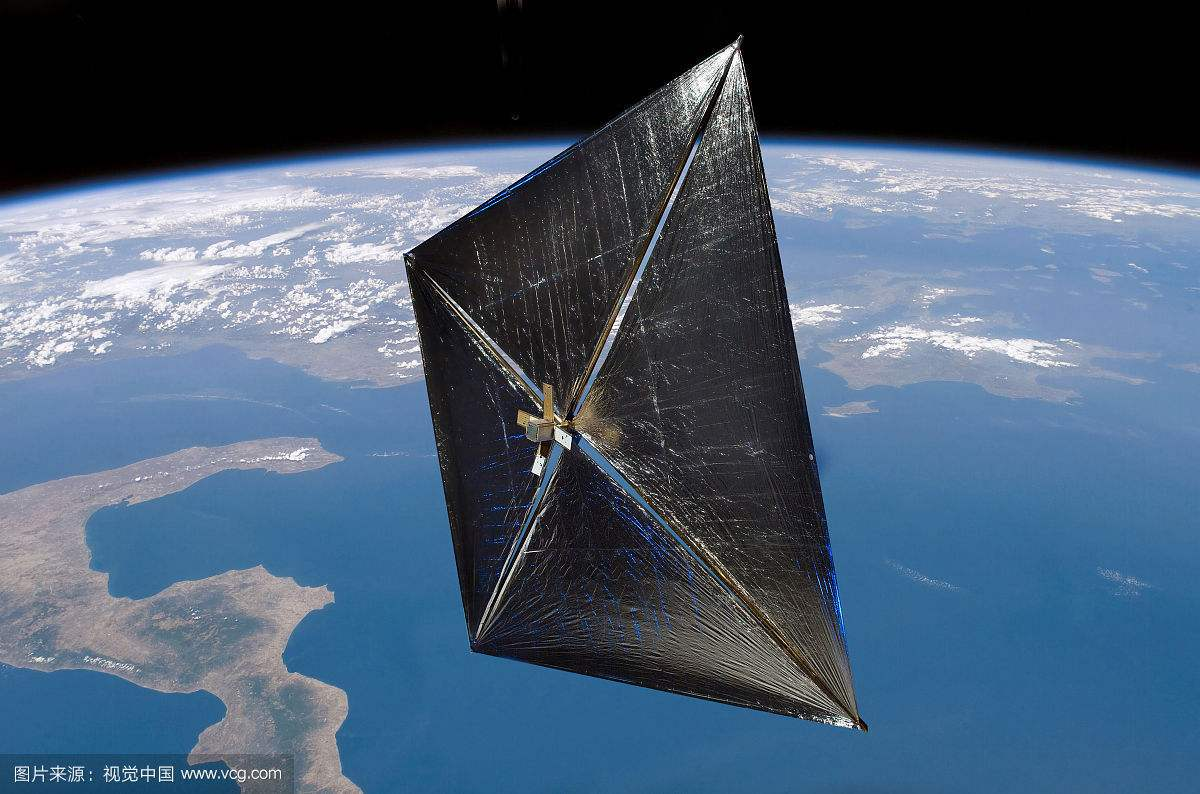
\includegraphics[scale=0.2]{../Figures/solarsailmodel.jpg}
 \caption{Solar sail}
\end{figure}

\begin{figure}[H]
\centering
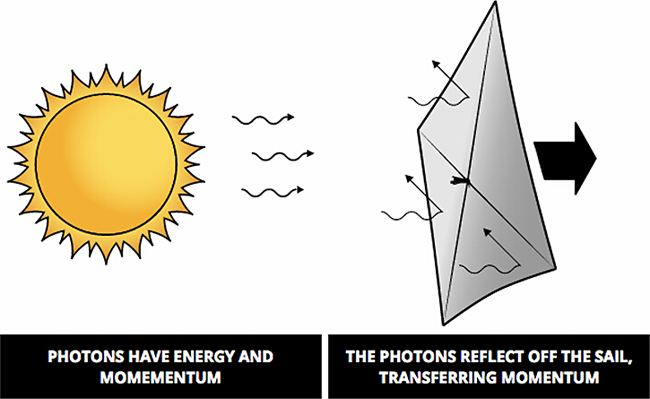
\includegraphics[scale=0.5]{../Figures/imagesolarsail.jpg}
\caption{Basic model of the solar sail}
\label{fig1}
\end{figure}
    
\subsection{Force of light pressure}

\subsubsection{Assumptions}

The following calculation of the force of light pressure is based on these three hypotheses:

(1)~The energy emitted by Sun during unit time is constant. 

(2)~The radiant energy absorbed by Mercury, Venus, and Earth is negligible;.

(3)~Only considered in the solar system.

\subsubsection{Calculation}

The solar constant (S.) refers to the solar radiation energy that received per second by per unit area of the top of the atmosphere circle perpendicular to the sunlight at the average distance from Sun to Earth ($D=1.496\times10^8km$). Similarly we denote S(r) as the energy flow density at the distance r from the Sun, and we denote $A$ as the area of solar sail.
\\

According to the conversation of energy:

\[S.\dfrac{4}{3}\pi{R_E}^2=S(r)\dfrac{4}{3}\pi r^2\]

\begin{equation}
S(r)=\dfrac{S.R_E^2}{r^2}
\end{equation}

The energy density is:\\
\begin{equation}
\rho_E=\dfrac{E}{V}=\dfrac{S.tAcos\alpha}{c tAcos\alpha}=\dfrac{S.}{c}
\end{equation}

The total light pressure is equal to twice of its energy density:
\begin{equation}
P(r)=2\rho_E=\dfrac{2S(r)}{c}=\dfrac{2S.{R_E}^2}{cr^2}
\end{equation}

The ideal plane solar sail model assumed that the impact of solar photon on the sail surface can be regarded as an ideal reflection, and the sail surface is an ideal plane. Therefore, the forces exert by incident photons and reflected photons are equal, shown as follows:

\begin{figure}[H]
 \centering
 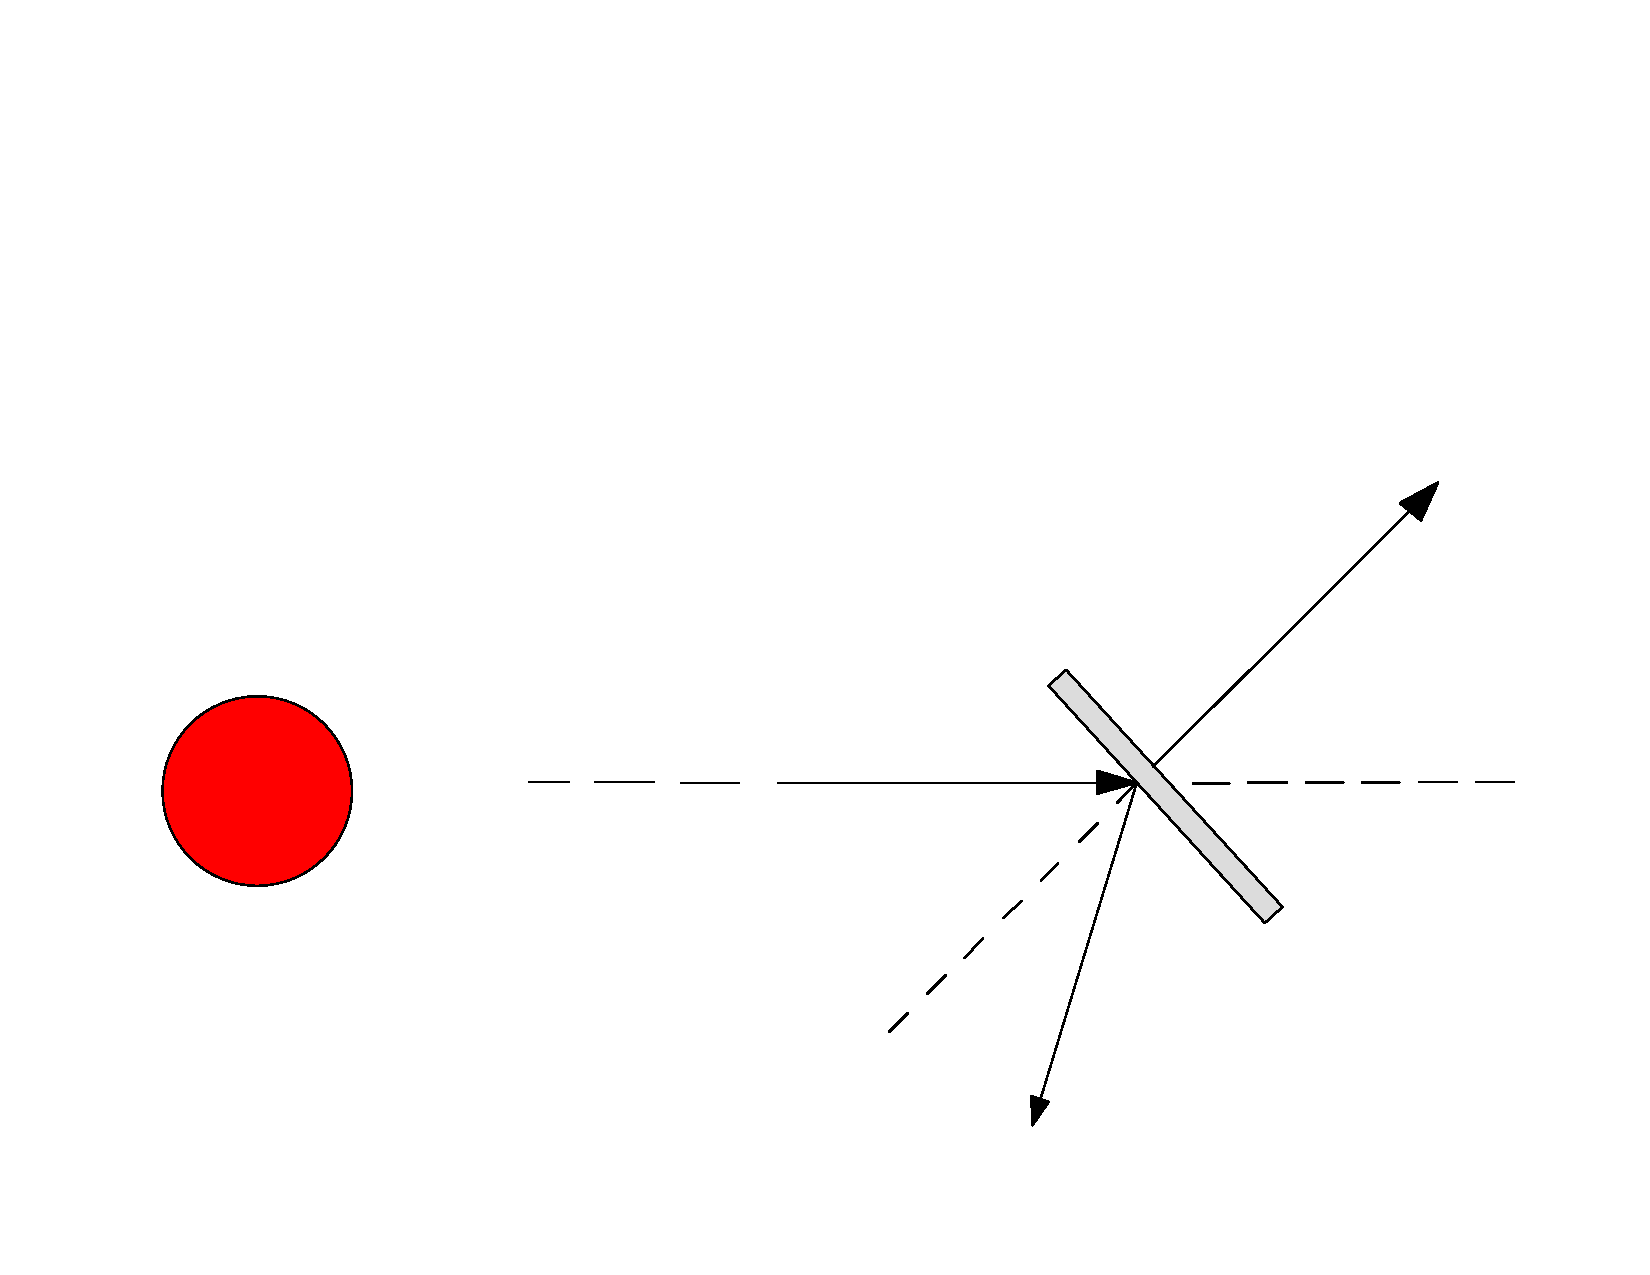
\includegraphics[scale=0.3]{../Figures/lightpressure.pdf}
 \caption{incident and reflected photon}
\end{figure}

The light pressure produced by the incident photon is:

\begin{equation}
P_i=\frac{P(r)}{2}A_z(cos\alpha~\vec{n}-sin\alpha~\vec{t})
\label{eq:1}
\end{equation}

In this formula, $A_z$ is the effective sail area, $\alpha$ is the angle between the incident ray and the solar sail unit normal direction $\vec{n}$, the unit vector of solar sail normal direction $\vec{n}$ is perpendicular to the sail plane and pointing out away from the sun. $\vec{t}$ is the tangent unit vector perpendicular to the normal $\vec{n}$, the anticlockwise direction is defined positive. Then the light pressure produced by the reflected light is as bellow:

\begin{equation}
P_r=\frac{P(r)}{2}A_z(cos\alpha~\vec{n}+sin\alpha~\vec{t})
\label{eq:2}
\end{equation}

The effective area refers to the area on which the sail is projected on the plane perpendicular to the sunlight, $A_z=Acos\alpha$. Therefore, the total light pressure acting on the ideal plane solar sail is:

\begin{equation}	
\vec{F_p}=\vec{F_i}+\vec{F_r}=P(r)Acos^2\alpha~\vec{n}=\dfrac{2S.{R_E}^2Acos^2\alpha}{cr^2}~\vec{n}
\label{eq:3}
\end{equation}

Therefore, the force of light pressure $F_p$ is always along the normal direction of solar sail surface, $\vec{f}=\vec{n}$, $\vec{f}$ is the unit vector of thrust, it is always in the direction along the pressure direction and deviates from the sun.

\subsection{Analysis of the gravitation}

We calculated the gravitation from the Sun, Earth, Mars when the spacecraft has not escaped the Earth and has not entered the orbit of Mars. It can be seen accorfing to the order of magnitude in figures bellow that during the process of flight, the gravitation exerted by the Earth and Mars both can be negligible in comparing to the Sun's gravity. Thus we can get a simplified model. 

%------------------太阳地球火星对航天器的引力关于r的变化相对大小 图----------------------%

\begin{figure}[H]
 \begin{minipage}[t]{0.5\linewidth}
 \centering{}
 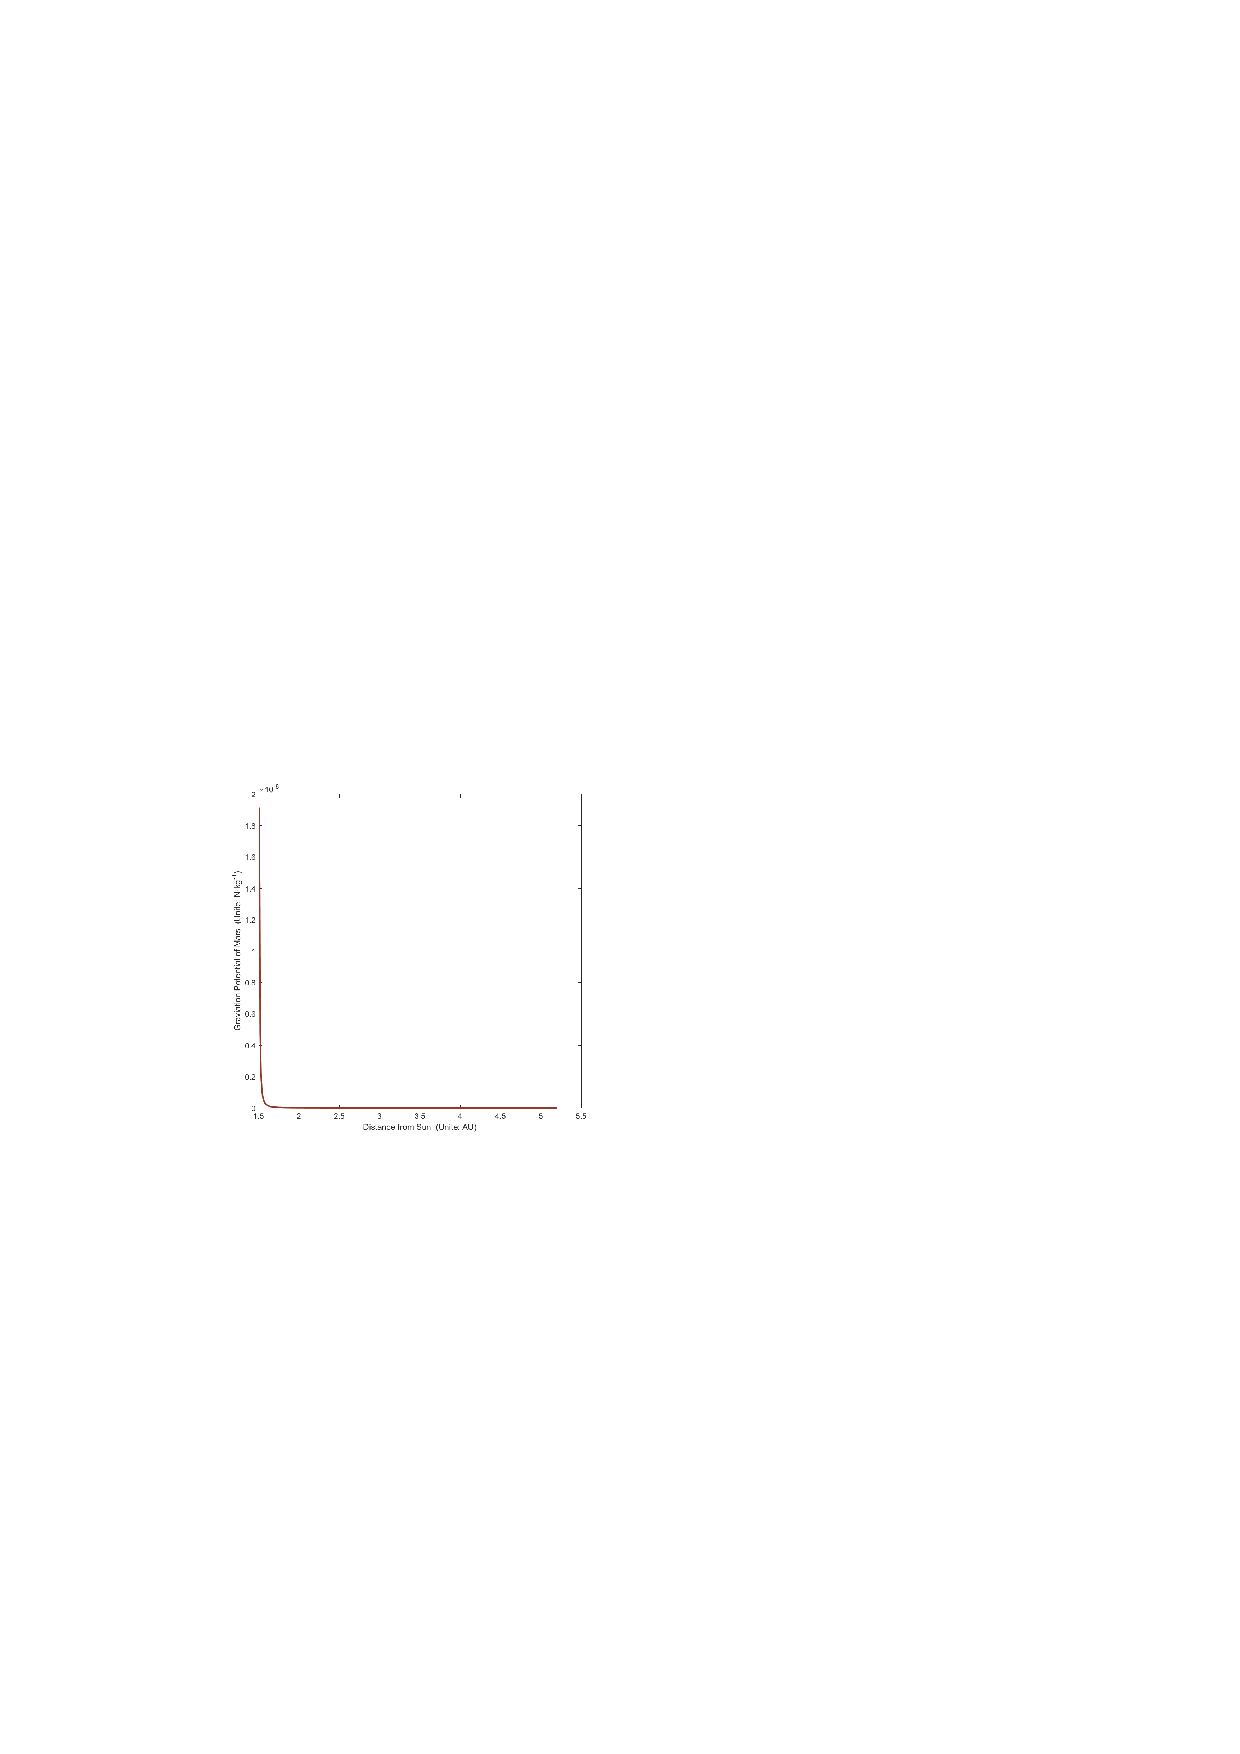
\includegraphics[width=7cm]{../Figures/gravmars.pdf}
 \label{fig:orbitlegend}
 \caption{Gravity of Mars}
 \end{minipage}
 \begin{minipage}[t]{0.5\linewidth}
 \centering{}
 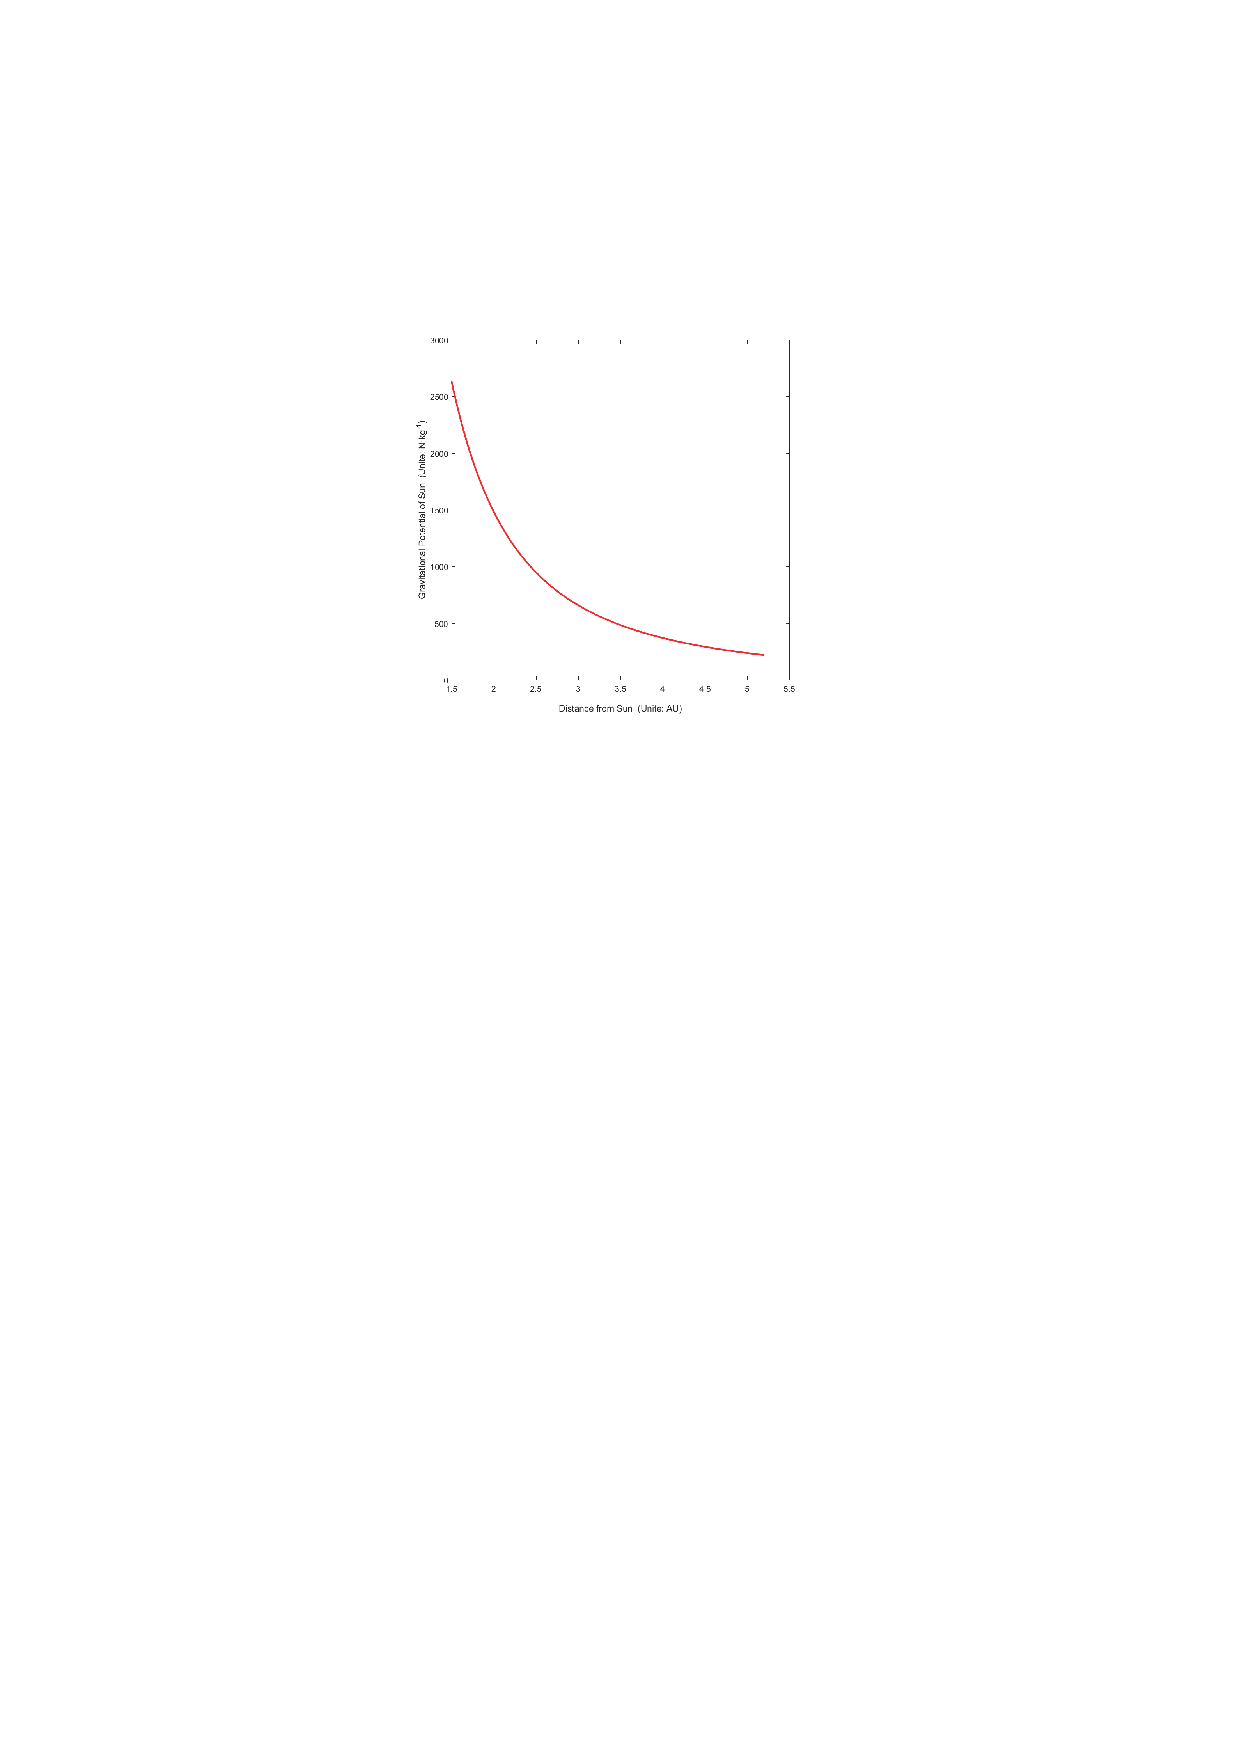
\includegraphics[width=7cm]{../Figures/gravsun.pdf}
 \label{fig:orbit1}
\caption{Gravity of Sun} 
 \end{minipage}
\end{figure}

\subsection{Force analysis and expression of acceleration}

In this problem, the solar sail is mainly affected by the gravity of Sun and the pressure of sunlight, because the magnitude of solar sail due to the gravitational action of Mercury, Venus and Earth is very small which can be neglected in comparing to the relative solar gravitation.

The solar sail is subjected to the small thrust from the continuous light pressure, and thrust itself is inversely proportional to the square of distance from Sun to the solar sail, so it can be realized with spiral trajectory.      

Light pressure is always deviated from the sun, by controling the attitude of solar sail, when the solar sail attitude angle $\alpha$ is positive, i.e. $F_p\cdot\alpha>0$, solar sail get orbital angular momentum, solar sail and spiral outward away from the sun; when the sail angle is negative, i.e. $F_p\cdot\alpha<0$, solar sail lose orbital angular momentum, and the solar sail moves toward the sun. 

\begin{figure}[H]
 \begin{minipage}[t]{0.5\linewidth}
 \centering{}
 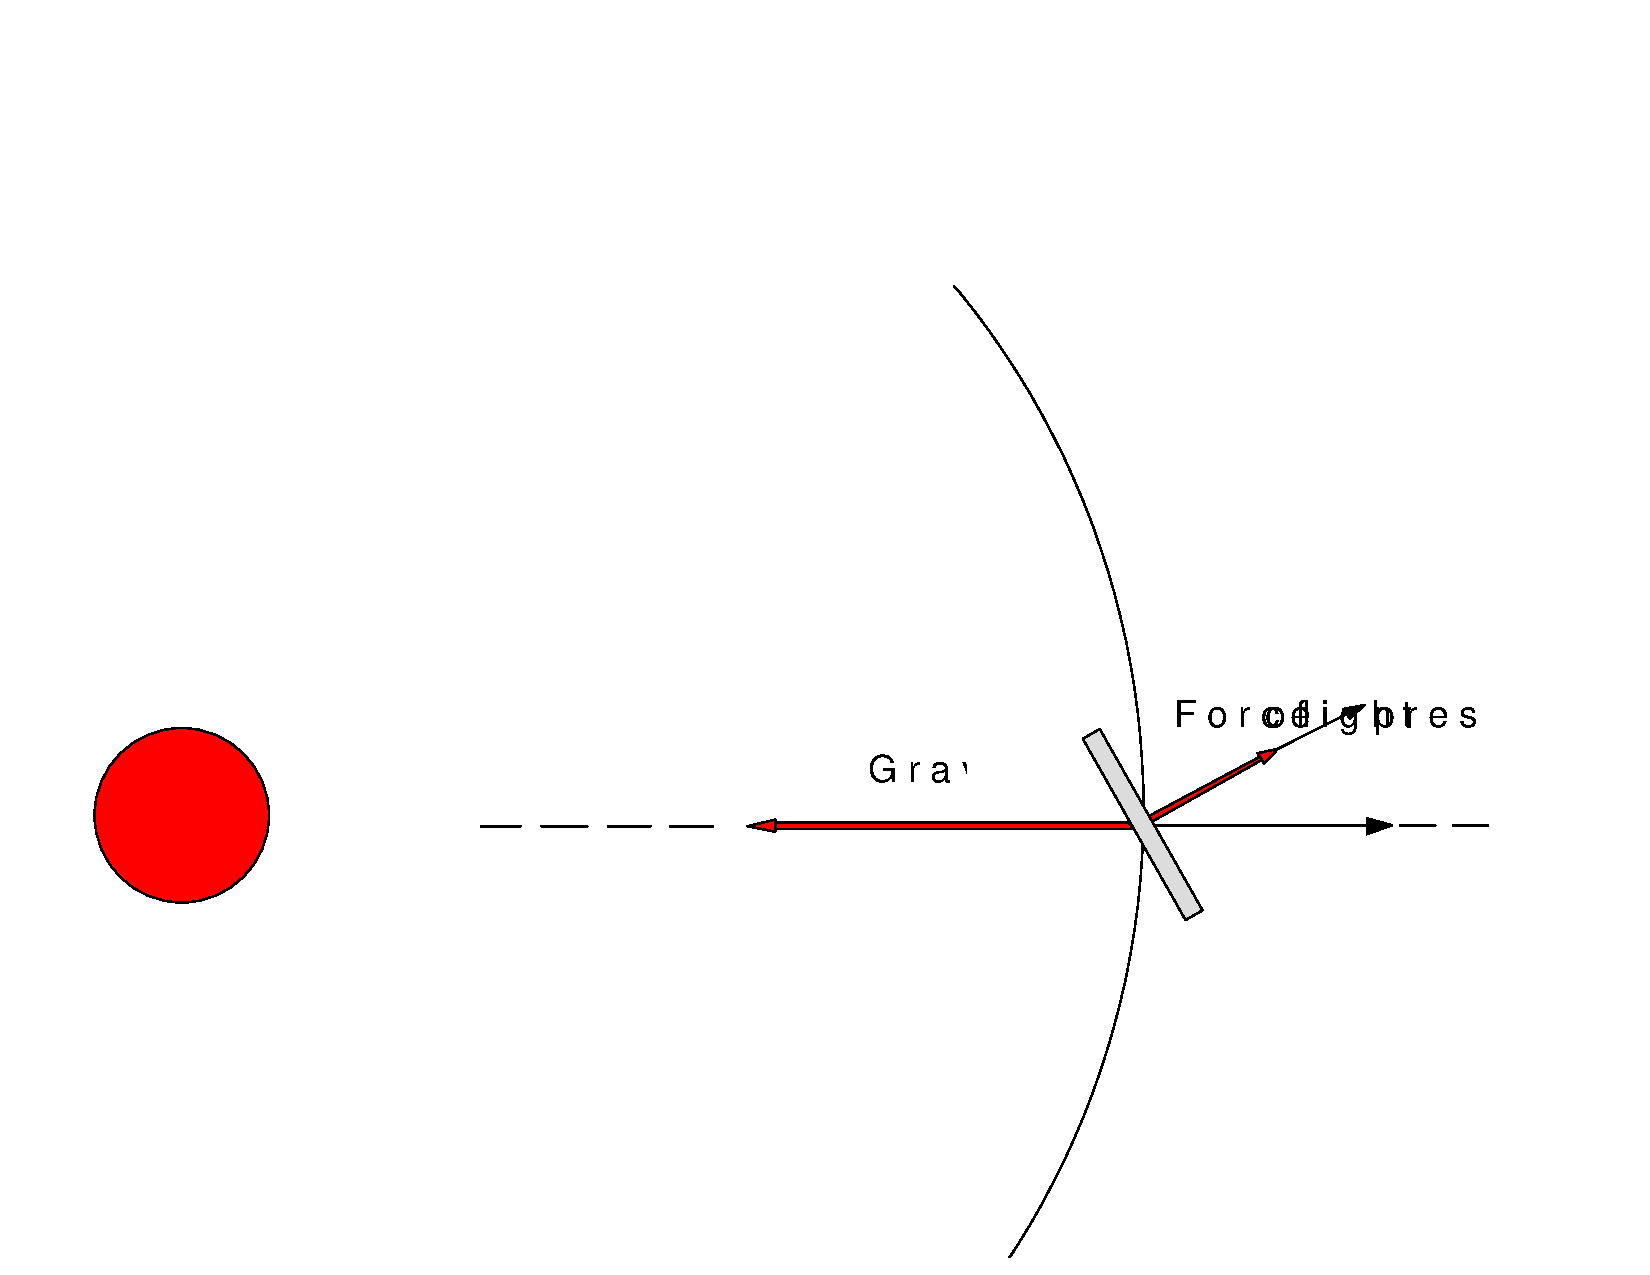
\includegraphics[scale=0.25]{../Figures/accelerate.pdf}
 \caption{spiraling outward($F_P\cdot\alpha>0$)}
 \label{fig:side:a}
 \end{minipage}
 \begin{minipage}[t]{0.5\linewidth}
 \centering{}
 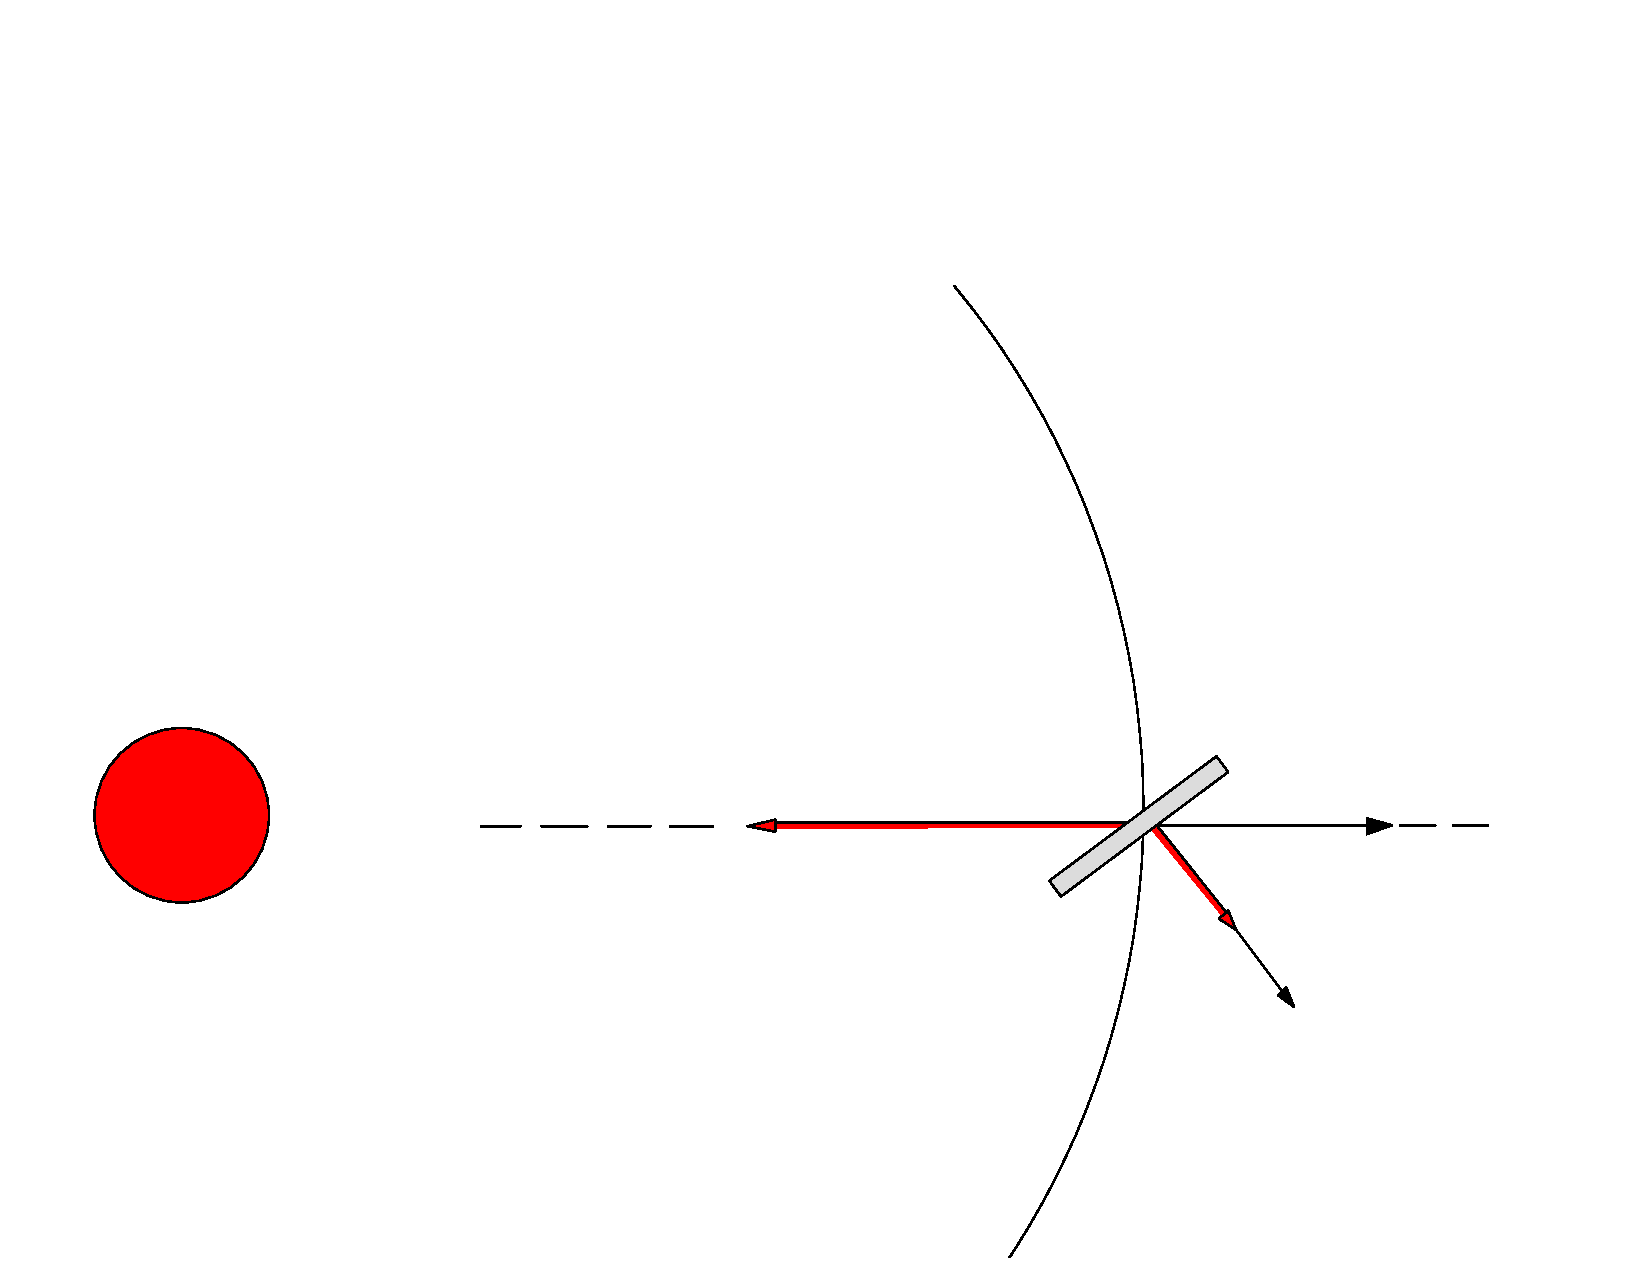
\includegraphics[scale=0.25]{../Figures/decrease.pdf}
 \caption{spiraling inward($F_P\cdot\alpha<0$)}
 \label{fig:side:b}
 \end{minipage}
\end{figure}

Denoted $F_g$ as the gravity of Sun received by solar sail and $\vec{F_g}=G\dfrac{M_Sm}{r^2}\vec{u_r}$.

According to the Newton Second Law:

\begin{equation}
\vec{F_g}+\vec{F_p}=m\vec{a}
\end{equation}

projected to the radial direction $\vec{u_r}$:

\begin{equation}
G\dfrac{M_Sm}{r^2}+\dfrac{2S.{R_E}^2Acos^2\alpha}{cr^2}\cdot cos\alpha=ma
\end{equation}

so we obtain the normal acceleration as:

\begin{equation}
\vec{a}=\left(\dfrac{GM_S}{r^2}+\dfrac{2S.{R_E}^2Acos^3\alpha}{mcr^2}\right)\vec{n}
\end{equation}

\subsection{Kinematical equation}

With the equation (2.6) when we suppose the surface of the solar sail is A, the attitude angle is $\alpha$ ( the attitude angle is defined by the included angle between the vector $\vec{n}$ and the vector $\vec{u_r}$ which have presented in the Figure.3) 

\begin{equation}
\vec{F_p} = P(r)Acos^2(\alpha)\vec{n}
\end{equation}

and the gravitation from the Sun:
\begin{equation}
\vec{F_g}=-\frac{GM_Sm}{r^2}\vec{u_r}
\end{equation}

We have the conversion relation between these vectors :
\begin{equation}
\vec{u_r}=cos\theta \vec{u_x} + sin\theta \vec{u_y}
\end{equation}

and
\begin{equation} 
\vec{u_\theta}=-sin\theta \vec{u_x} + cos\theta \vec{u_y}
\end{equation}

so the normal should be:
\begin{align*}
\vec{n} &= cos\alpha \vec{u_r} + sin\alpha \vec{u_\theta}\\
	    &= cos\alpha (cos\theta \vec{u_x} + sin\theta \vec{u_y}) + sin\alpha (-sin\theta \vec{u_x} + cos\theta \vec{u_y})\\
	    &=(cos\alpha cos\theta - sin\alpha sin\theta )\vec{u_x} + (cos\alpha sin\theta + sin\alpha cos\theta)\vec{u_y} 
\end{align*}

Then we project this two force to the axe x and axe y:
\begin{equation}
\vec{F_x} = (-\frac{GMmx}{(\sqrt{x^2+y^2})^3} + \dfrac{C_{1} A cos^2 \alpha}{\sqrt{x^2+y^2}} (cos\alpha\frac{x}{\sqrt{x^2+y^2}} - sin\alpha\frac{y}{\sqrt{x^2+y^2}}))\vec{u_x}
\label{eq:diffx}
\end{equation}

\begin{equation}
\vec{F_y} = (-\frac{GMmy}{(\sqrt{x^2+y^2})^3} + \dfrac{C_{1} A cos^2 \alpha}{\sqrt{x^2+y^2}} (cos\alpha\frac{y}{\sqrt{x^2+y^2}} + sin\alpha\frac{x}{\sqrt{x^2+y^2}}))\vec{u_y}
\label{eq:diffy}
\end{equation}

Where $C_1 = 2.04 \times 10^11 $ is a coefficient about light pressure.

According to the basic principle of dynamics, we can get these kinematical equation:

\begin{equation}
\frac{d^2x}{dt^2} = \frac{F_x}{m}
\end{equation}
\begin{equation}
\frac{d^2y}{dt^2} = \frac{F_y}{m}
\end{equation}

After we finish the basic kinematical equation, we can use MATLAB to solve with initial conditions to get its trajectory.

\subsection{Trajectory}

\subsubsection{Assumption}

Here, we make some simplificaition in considering the orbits: 
%在轨道的考虑上我们做了一些简化:

(1) these revolution orbits of Earth and Mars are periphery,          
%(1) 火星地球做公转的轨道是圆周轨道;

(2) these revolution plane of Earth and Mars is the same plane.   
%(2)火星地球公转的轨道平面在同一平面。

\subsubsection{The initial state of the solar sail spacecraft}

First, considering that the solar sail spacecraft will be launched from Earth to Mars, and it needs to use the rocket to accelerate the spacecraft to Earth's escape velocity. The best and most fuel-efficient situation here is that the energy that solar sails spacecraft is given by the rocket is just enough to get the spacecraft out of the Earth's gravitational field, so, we are treating the speed of the solar sail with the speed of the Earth's revolution speed  and direction.

Next we consider the mass of the spacecraft is 2000kg.

\subsubsection{Trajectory without power}

According to the initial condition, without the power and the influence of the gravitation from Earth, it is simple to understand that the trajectory of spacecraft is the revolutionary orbit.

\subsubsection{Trajectory with power}

In this section we have got some trajectories of the spacecraft by setting the value of surface area A of the solar sail and the attitude angle $\alpha$. We can figure out that if we want to send the solar sail to Mars or outer planet, we have to make the attitude angle positive ($\alpha > 0$),  i.e. the situation: spiraling outward. And the other situation is spiraling inward ($\alpha < 0$) which is corresponding to sending the solar sail to inner planet e.g. Mercury. We want to change the surface area A and the attitude angle $\alpha$ to make it to the revolutionary orbit of Mars. The test verifies that the spacecraft can indeeds get to the revolutionary orbit of Mars, i.e. sending the equipment to Mars by using the solar sail is absolutely viable in some conditions.

%--------------需要至少两个图两个姿态角为正,一个姿态角为负----------------%

%在这一部分,通过设置不同的太阳帆表面积和姿态角,得到了一些航天器的轨迹曲线,从图中可以看出从地球向火星或者说外星系发射太阳帆航天器,姿态角必须是正角,也就是在4.4部分所说的加速情况,而向内星系比如说水星,就是另外一种情况(姿态角为负数的情况)。我们想改变太阳帆表面积及姿态角让航天器能够到达火星轨道,试验的结果证明:在一定的条件下,航天器的轨迹可以到达火星轨道,也就是说,通过太阳帆将仪器设备或者其他载荷送到火星绝对是可行的。

\begin{figure}[H]
\centering
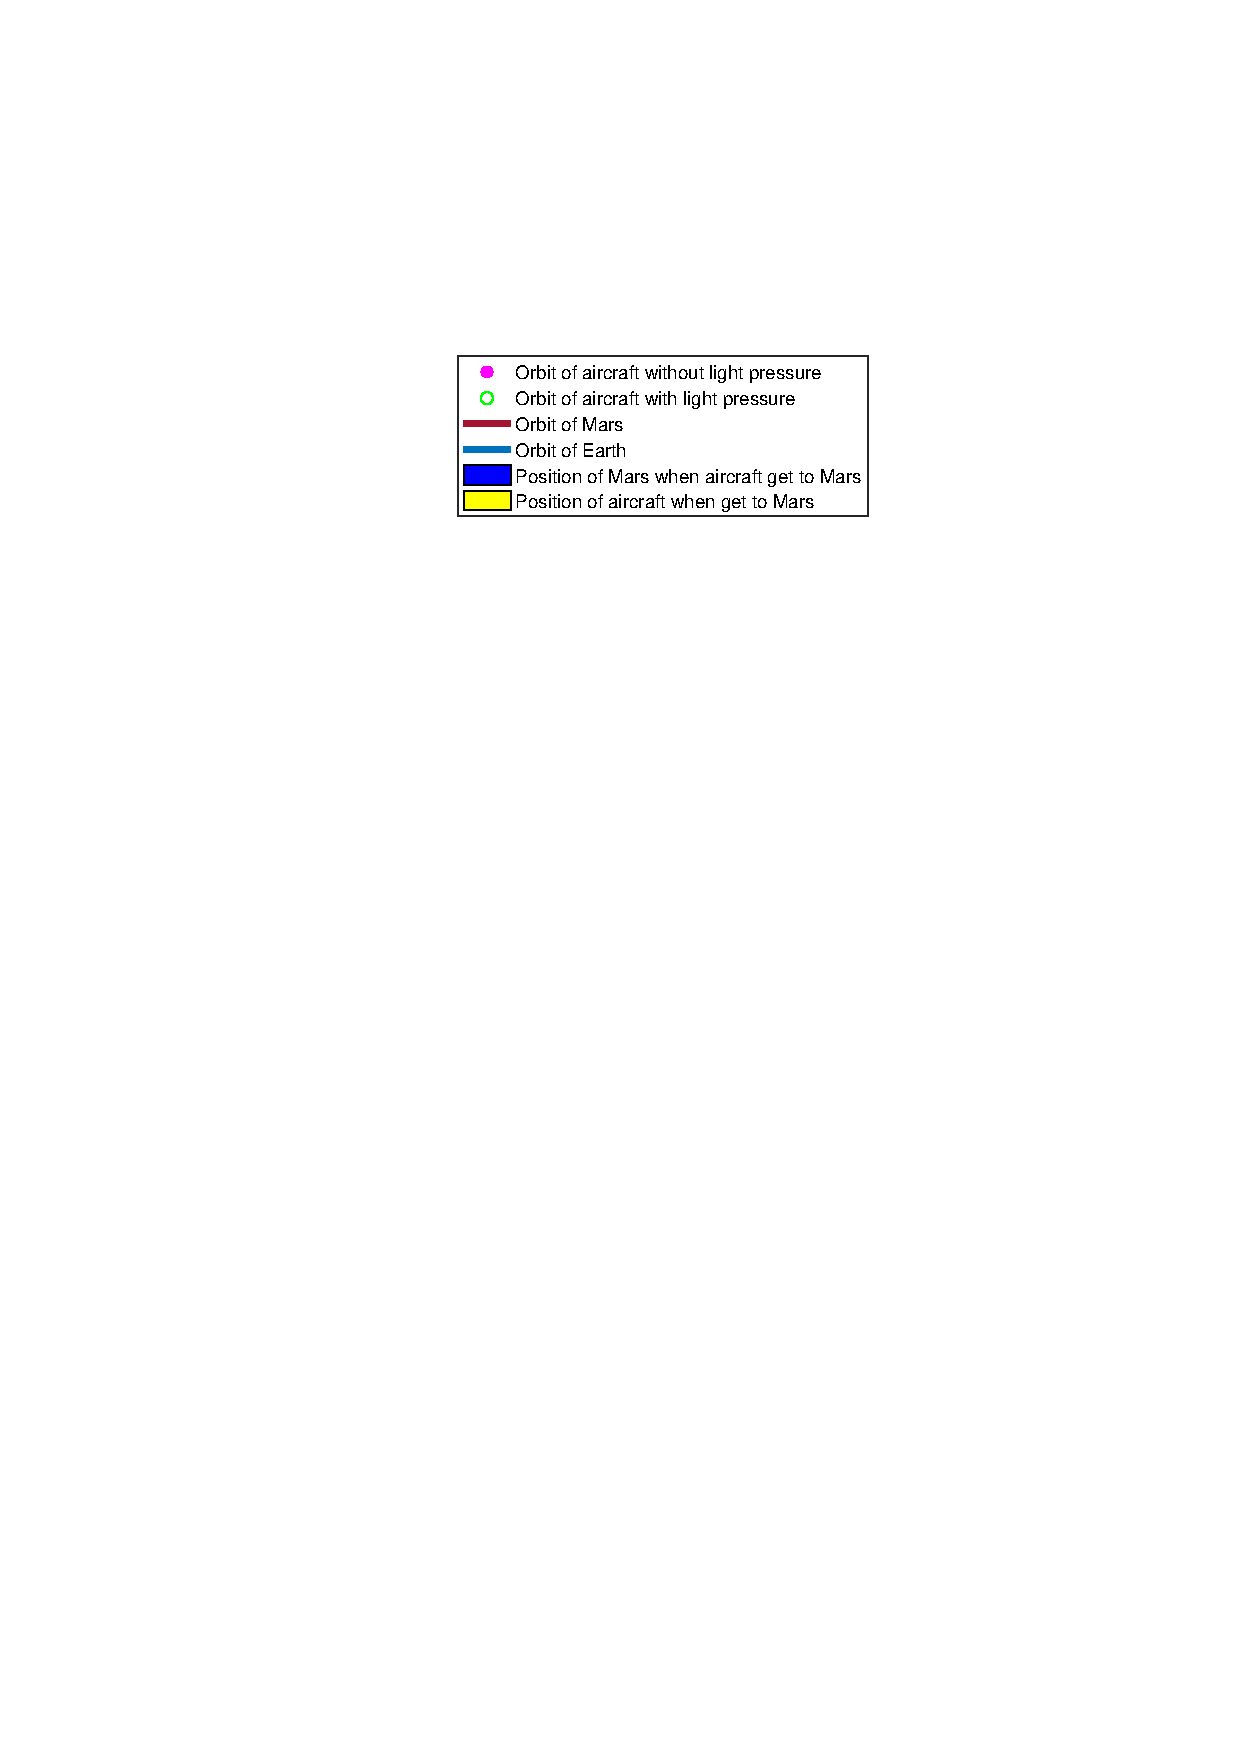
\includegraphics[width=8cm]{../Figures/label_of_7_orbits.pdf}
\caption{Legend of Lines and Points in figures below}
\end{figure}

\begin{figure}[H]
 \begin{minipage}[t]{0.5\linewidth}
 \centering{}
 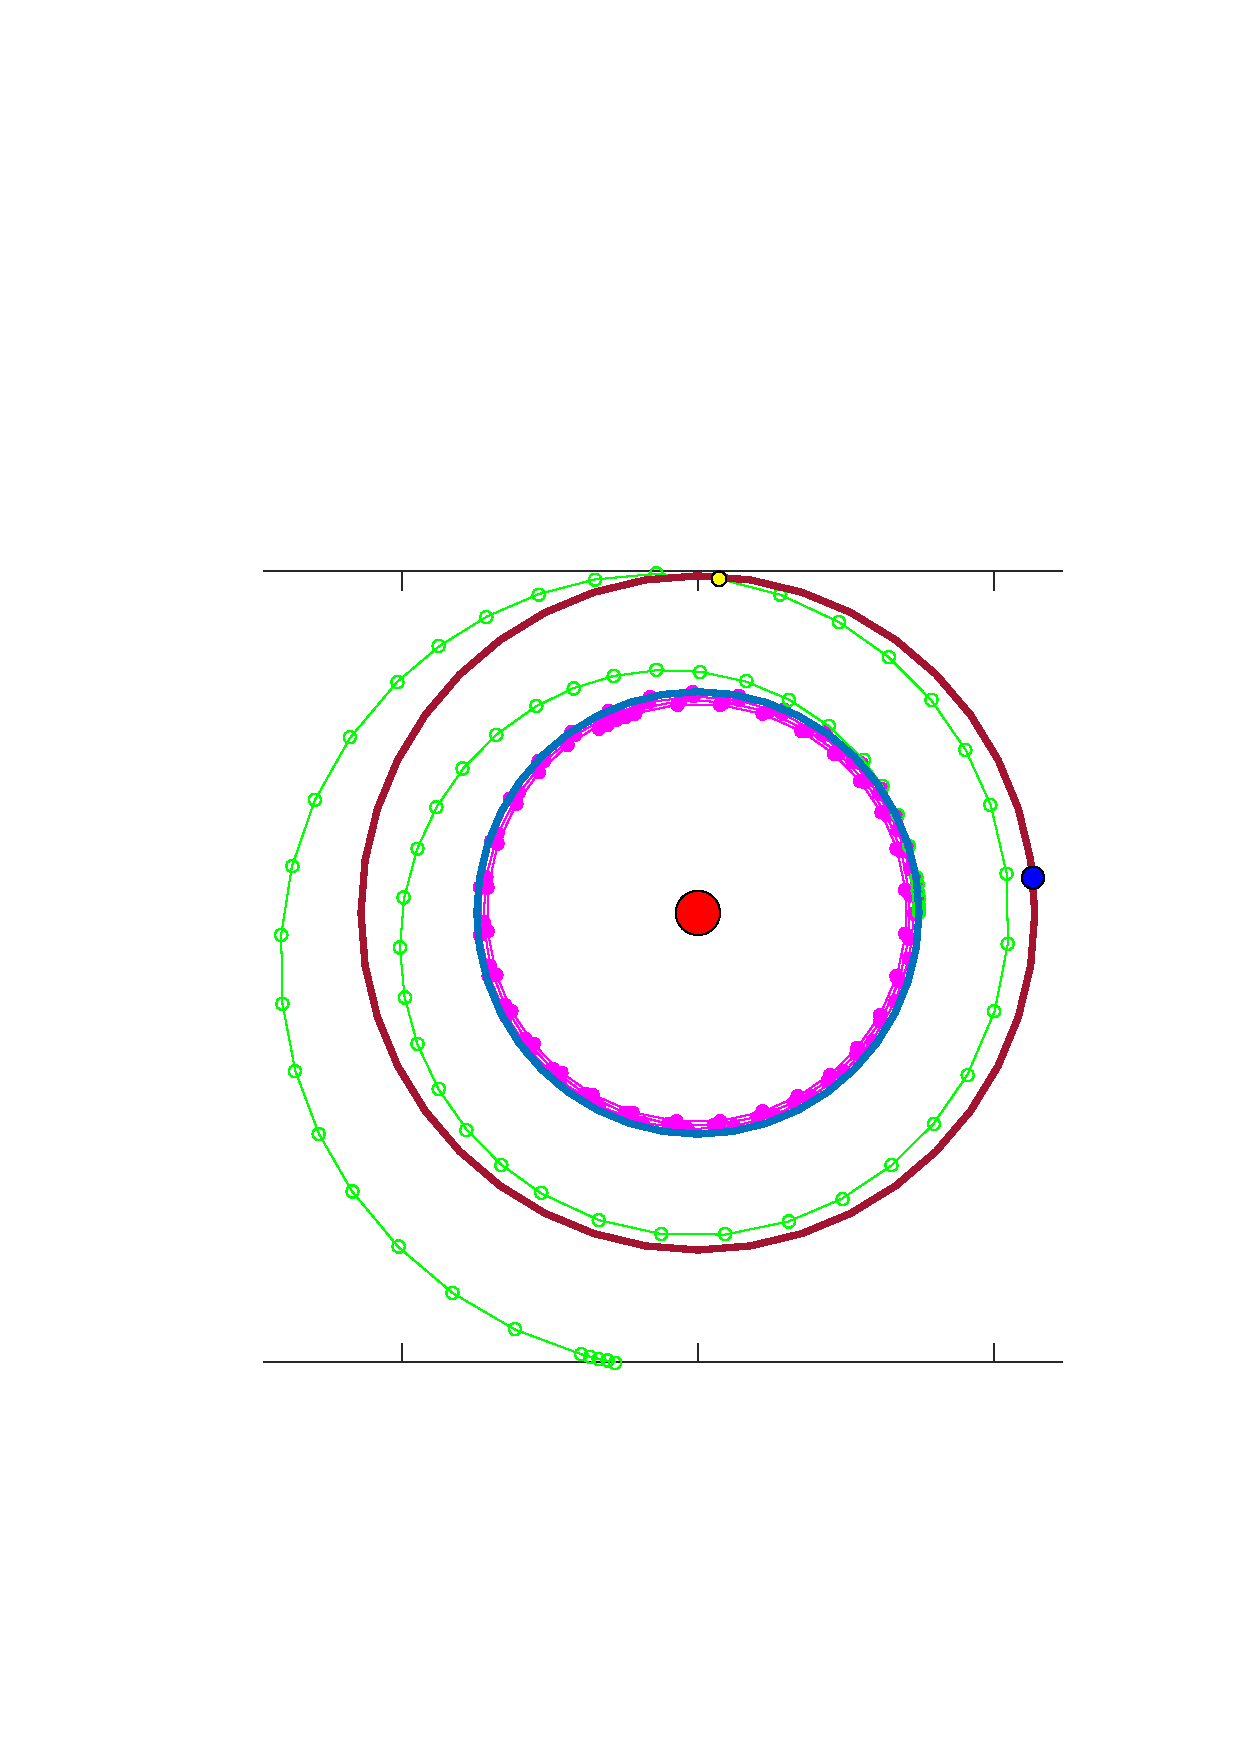
\includegraphics[width=7cm]{../Figures/alphadayu0.pdf}
 \label{fig:orbitlegend}
 \caption{$\alpha > 0$}
 \end{minipage}
 \begin{minipage}[t]{0.5\linewidth}
 \centering{}
 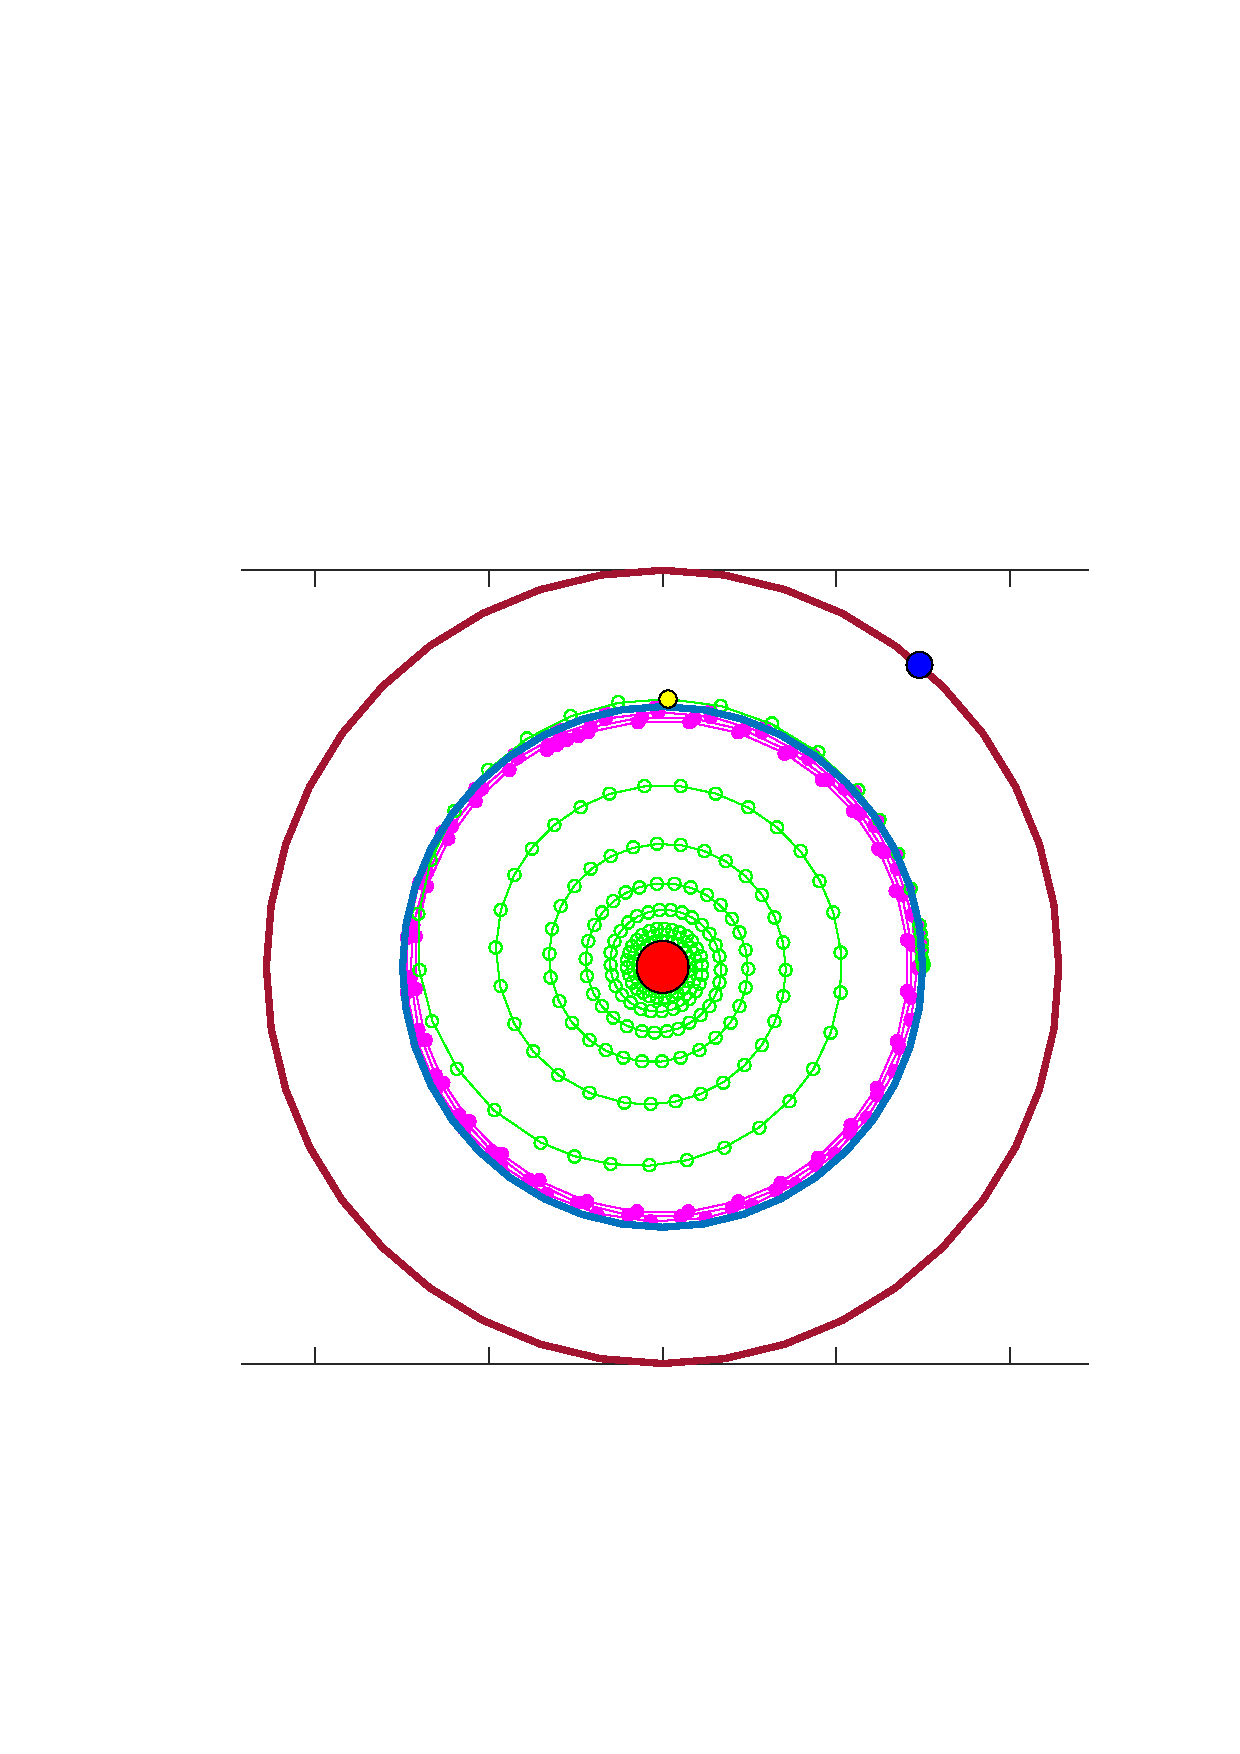
\includegraphics[width=7cm]{../Figures/alphaxiaoyu0.pdf}
 \label{fig:orbit1}
\caption{$\alpha < 0$}
 \end{minipage}
\end{figure}

\end{document}